\section{The two literatures}
\label{sec:literatures}

This section exists to establish one fact: the experiment this paper runs has
never been run. Everything in it is measurement over a corpus, and it ends at
the cell of the matrix that is empty.

\subsection{Corpus}

We began from 51 seed papers found during scoping, queried the Semantic
Scholar Academic Graph and arXiv APIs with keyword clusters drawn from both
vocabularies, and snowballed forward and backward. The discovery pool reached
25,922 papers. Dual coding at that scale is not feasible for a small team, so
we screened on title and abstract against written inclusion criteria, then read
the survivors in full. The included corpus is \NCorpus{} papers, each carrying
\NColumns{} recorded columns of which \NCodedFields{} are coded from the full
text.

\begin{figure}[t]
\centering
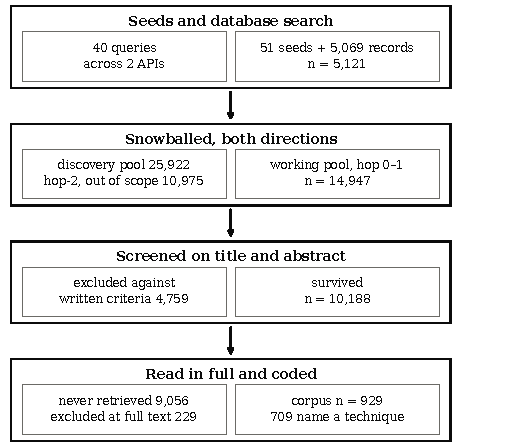
\includegraphics[width=\columnwidth]{figures/fig9_prisma}
\caption{Corpus construction, counted at every stage. One edge is honest
about a gap: the records that survived screening but were never retrieved
were chosen by a rule the project did not record. The queries, their dates
and their hit counts ship with the artifact as a search log.}
\label{fig:prisma}
\end{figure}

Figure~\ref{fig:prisma} counts every stage, and the artifact ships the
\NQueries{} queries with their dates and hit counts. One stage is weaker than
the rest. Of the \NSurvived{} records that survived screening,
\NFullText{} were read in full, and nothing we recorded says how that subset
was chosen. We report the gap rather than reconstruct a rule for it.

Screening changed the corpus three times during the project and we report the
current state only; every change is logged. The most recent was a
contribution re-screen in which all \NScreened{} screened papers were re-read
against a single rule: a paper stays if it contributes an attack, a failure
mechanism, a defense or a fix. Benchmarks, surveys, measurement studies and
position papers are kept even though they propose no technique, because they
are how the field is organized. That pass removed 53 papers and, in the other
direction, recovered 34 techniques that the original extraction had missed, so
the registry counts in this paper are floors rather than censuses.

\subsection{A joint taxonomy}
\label{sec:taxonomy}

We place every named mechanism and every named defense on three axes. Each
axis value is named by the work that first identified it as a distinct
surface or a distinct harm; we group the names rather than coin them. The axes let the two
literatures land in the same space without forcing them into the same words. A
security attack and a machine learning mechanism that enter by the same route
and cause the same damage occupy the same cell. They differ only on intent. That is what makes the taxonomy a way of finding missing
experiments rather than a filing scheme.

\textbf{Channel} is the route untrusted content takes into the context window.
There are nine. \meth{direct-input} is content placed in the prompt by the user
or an upstream service~\cite{liu-2023-promptb}. \meth{RAG} is a passage a retriever selected from a
corpus~\cite{zhong-2023-poisoning,zou-2024-poisonedrag}. \meth{tool-output} is whatever a called tool returned~\cite{greshake-2023-not}.
\meth{tool-metadata} is the names, descriptions and schemas of the tools
themselves, which the model reads before it calls anything~\cite{shi-2025-prompt}. \meth{memory} is
what the agent stored from an earlier turn or session~\cite{chen-2024-agentpoison}. \meth{skill} is a file or
instruction set the agent loads to extend itself~\cite{schmotz-2025-agent}. \meth{multi-agent} is a
message from another agent~\cite{chen-2023-scalable}. \meth{cross-modal} is content that arrives as an
image, audio or document and is rendered into text~\cite{zhu-2024-unraveling}. \meth{supply-chain} is
content entering through a package, template or model the agent depends
on~\cite{yan-2023-backdooring}.

\textbf{Intent} is whether the content was placed deliberately: adversarial,
incidental, or studied as both.

\textbf{Consequence} is what the agent then does wrong. There are six.
\meth{goal-hijack} is pursuing an objective it was not
given~\cite{greshake-2023-not}.
\meth{reasoning-corruption} is reaching a wrong conclusion while pursuing the
right goal~\cite{liu-2023-lost}. \meth{silent-corruption} is producing a wrong output with nothing
to signal it~\cite{zhong-2023-poisoning}. \meth{data-exfiltration} is information crossing a boundary it
should not~\cite{yu-2023-assessing}. \meth{persistence-backdoor} is corruption that survives into a
later session~\cite{yan-2023-backdooring}. \meth{resource-abuse} is spending compute, money or quota on the
attacker's behalf~\cite{debi-2026-whispers,feiglin-2026-benchoverflow}.

The three axes give \NCubeCells{} cells. The consequence axis gained
\meth{availability-loss} after a full-text re-coding pass found papers whose
measured harm is the agent failing to finish at all, which the original six
could not express. Adding a sparse column raises the share of empty cells
without anything in the field having changed, and we report the figure on the
larger grid rather than the smaller one it would flatter.

\NUnplaceable{} papers (\PctUnplaceable{}\%) carry no single channel or
consequence. These are surveys and benchmarks whose attack surfaces are
co-equal by construction, and forcing one coordinate on them would invent
precision. They are counted in the corpus and excluded from the cube.

\begin{figure*}[t]
\centering
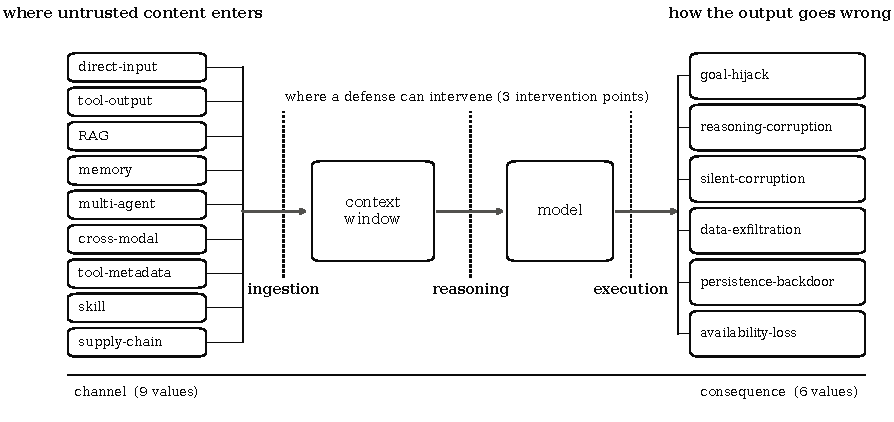
\includegraphics[width=\textwidth]{figures/fig0_pipeline}
\caption{The taxonomy against the system it describes. Untrusted content
arrives through one of nine \textbf{channels}, enters one context window, and
the output fails as one of six \textbf{consequences}. A defense can intervene
at three points, and the two literatures do not choose the same one: the
security track masses at ingestion, the machine learning track at reasoning,
and execution is security almost alone. Counts are named mechanisms per
channel (left) and named defenses per intervention point (center) and named mechanisms per
consequence (right), by track. The consequence column is the sharpest
division in the figure: goal-hijack is security-track \NGoalHijackSec{} to
\NGoalHijackML{}, and reasoning corruption runs the other way, \NReasonML{}
to \NReasonSec{}.
Drawn as a flow rather than a tree because the taxonomy is a cube; the
pipeline is the one ordering the three axes genuinely have.}
\label{fig:pipeline}
\end{figure*}

Figure~\ref{fig:pipeline} puts the three axes against the system they
describe, and shows a separation the axes alone do not.

The two literatures intervene at different points of the same pipeline.
Security defenses mass at ingestion, where the question is whether content
should be admitted. Machine learning fixes mass at reasoning, where the
question is what to believe once it has been admitted. Execution, where the
question is what the agent is then permitted to do, is security almost alone.
The split is not only in vocabulary; it is in where each community thinks the
problem should be solved, and a method built for one point is not a drop-in at
another.

The consequence axis separates them even more sharply, and the registry says
so outright. Of the \NMechGoalHijack{} named goal-hijack mechanisms,
\NGoalHijackSec{} come from the security track and \NGoalHijackML{} from
machine learning. Reasoning corruption runs the other way, \NReasonML{} to
\NReasonSec{}. That is not two communities describing one phenomenon in different
words. It is two communities that have divided the phenomenon between them and
stopped at the boundary.

% GENERATED by scripts/gen_taxonomy_tables.py -- do not hand-edit.
\begin{table*}[t]
\centering
\caption{Named mechanisms per channel, by track, with the most-tested examples each literature contributes. Counts are named mechanisms in the registry; examples exclude entries whose authors named nothing, and are ordered by how many defenses have been evaluated against them. The channels both communities name are the first four rows; the last five are named by the security literature almost alone.}
\label{tab:channels}
\small
\begin{tabular}{@{}lrrp{0.31\textwidth}p{0.31\textwidth}@{}}
\toprule
\textbf{Channel} & \textbf{Sec} & \textbf{ML} & \textbf{Security names} & \textbf{Machine learning names} \\
\midrule
\meth{tool-output} & 64 & 3 & Indirect Prompt Injection~\cite{greshake-2023-not}; BIPIA benchmark attack set~\cite{yi-2023-benchmarking}; Neural Exec~\cite{pasquini-2024-neural} & context rot~\cite{xia-2026-diagnosing}; observation over-ingestion~\cite{gaur-2026-signaldriven}; plan anchor~\cite{yu-2026-webanchor} \\
\meth{direct-input} & 36 & 31 & Combined Attack~\cite{liu-2023-formalizing}; HackAPrompt: prompt-hacking t\,…~\cite{schulhoff-2023-ignore}; Tensor Trust: prompt extracti\,…~\cite{toyer-2023-tensor} & lost in the middle~\cite{liu-2023-lost}; distraction by irrelevant con\,…~\cite{shi-2023-large}; context drift~\cite{dongre-2025-drift} \\
\meth{RAG} & 24 & 6 & PoisonedRAG~\cite{zou-2024-poisonedrag}; Indirect Data Poisoning~\cite{gyevnar-2026-distributed}; Salience Induction~\cite{zhou-2026-salience} & distraction by irrelevant con\,…~\cite{wu-2024-easily}; identity drift~\cite{platnick-2025-idrag}; context compliance~\cite{chen-2026-rag} \\
\meth{cross-modal} & 15 & 4 & steganographic prompt injecti\,…~\cite{pathade-2025-invisible}; MIRAGE~\cite{dai-2026-mirage}; WebInject~\cite{wang-2025-webinject} & evidence misalignment~\cite{qiu-2026-videoseal}; cross-modality parametric kno\,…~\cite{zhu-2024-unraveling}; context unawareness~\cite{xu-2026-contextaware} \\
\meth{memory} & 11 & 7 & Cross-Session Stored Prompt I\,…~\cite{xie-2026-prompt}; AgentPoison~\cite{chen-2024-agentpoison}; MemoryGraft~\cite{srivastava-2025-memorygraft} & memory misevolution~\cite{xie-2026-memevobench}; memory pollution~\cite{liu-2026-failuregated}; memory laundering~\cite{wang-2026-state} \\
\meth{tool-metadata} & 11 & 1 & Cross-Tool Description Poison\,…~\cite{shi-2026-think}; ChatInject~\cite{chang-2025-chatinject}; Branded Whisper Attack / Vaul\,…~\cite{debi-2026-whispers} & context rot~\cite{ayyagari-2026-context} \\
\meth{multi-agent} & 6 & 3 & PlanFlip~\cite{wang-2026-planflip}; OMNI-LEAK~\cite{naik-2026-omnileak}; Prompt Infection~\cite{lee-2025-prompt} & Constraint Drift~\cite{bui-2026-himaptravel}; extraneous cognitive load~\cite{shang-2025-united}; context poisoning~\cite{chen-2026-unlocking} \\
\meth{supply-chain} & 6 & 0 & PoisonedSkills / DDIPE~\cite{qu-2026-supplychain}; Parasitic Toolchain Attacks~\cite{zhao-2025-parasites}; Virtual Prompt Injection (VPI)~\cite{yan-2023-backdooring} & --- \\
\meth{skill} & 3 & 1 & SkillJect~\cite{jia-2026-skillject}; POISE~\cite{hao-2026-poise} & --- \\
\bottomrule
\end{tabular}
\end{table*}


\textbf{What is in the cells.} Table~\ref{tab:channels} names what each
literature actually contributes per channel, because a count of
\NMechanisms{} mechanisms is not a description of them. Four channels are named
by both communities and five are effectively security-only:
\meth{supply-chain} has no machine learning entry at all, and
\meth{tool-metadata} and \meth{skill} have one each. \meth{tool-output} is the
most lopsided channel in the corpus, and \meth{direct-input} the only balanced
one.

\meth{memory} is the clearest case of the same ground named twice. The security literature contributes
AgentPoison~\cite{chen-2024-agentpoison},
MemoryGraft~\cite{srivastava-2025-memorygraft} and Sleeper Memory Poisoning;
the machine learning literature contributes memory pollution, memory laundering
and multi-target interference. Same channel, adjacent words, two literatures.

\begin{figure}[t]
\centering
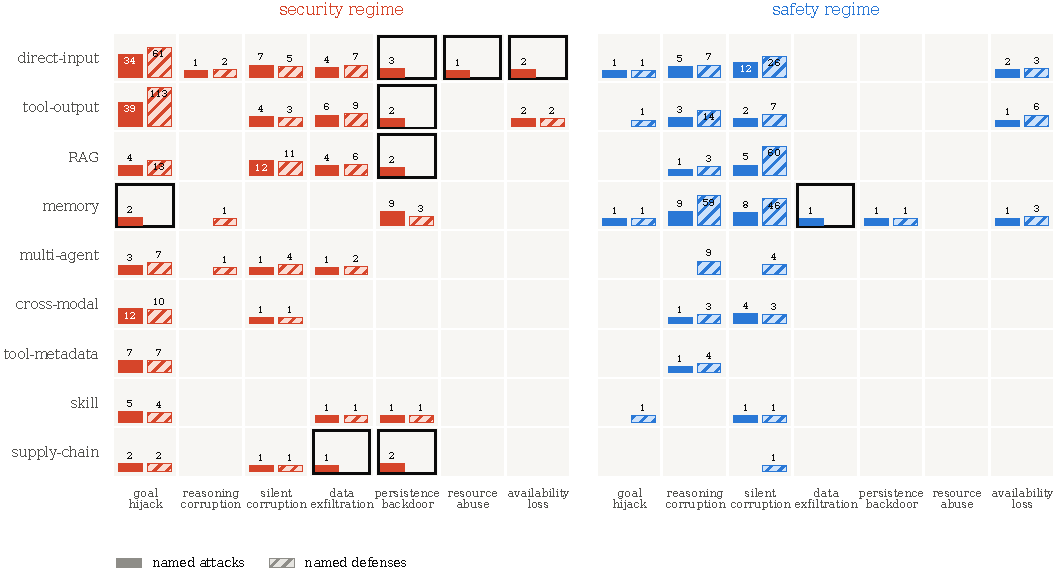
\includegraphics[width=\columnwidth]{figures/fig1_cube}
\caption{Channel $\times$ consequence occupancy, split by track. Empty cells
are hatched rather than shaded, because the claim is about which cells hold no
paper at all.}
\label{fig:cube}
\end{figure}

\textbf{\NCubeEmpty{} of the \NCubeCells{} cells (\PctCubeEmpty{}\%) contain no
paper from either literature.} Emptiness is not uniform. Figure~\ref{fig:cube}
shows the two tracks concentrating in different columns. The cells
empty in both tracks are the ones where neither community has looked, which is
a different and more interesting gap than a cell one community has to itself.

Figure~\ref{fig:channelgap} asks a separate question: where protection does not
follow the problem. Counting named defenses against named mechanisms per
channel, \meth{multi-agent} and \meth{memory} are served at roughly four
defenses per mechanism, while \meth{supply-chain} has fewer defenses than
mechanisms and \meth{cross-modal} and \meth{tool-metadata} sit at parity. Those
three are the routes by which an agent accepts capability from a third party,
and they are the thinnest in the corpus.

\begin{figure}[t]
\centering
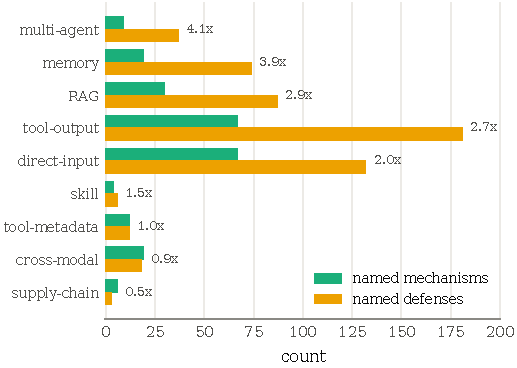
\includegraphics[width=\columnwidth]{figures/fig2_channel_gap}
\caption{Named mechanisms against named defenses, per channel, labeled with
defenses per mechanism. Channels are ordered by that ratio, so the under-served
routes fall to the bottom. \meth{supply-chain} has fewer defenses than named
mechanisms; \meth{cross-modal} and \meth{tool-metadata} are at parity. These
are the routes by which an agent accepts third-party capability.}
\label{fig:channelgap}
\end{figure}

\textbf{Census.} The registry holds \NMechanisms{} named mechanisms,
\NMechSecurity{} from the security track and \NMechML{} from the machine
learning track, and \NDefenses{} named defenses and fixes, \NDefSecurity{}
and \NDefML{} respectively with \NDefBoth{} claimed by both. By consequence,
\meth{goal-hijack} dominates the threat side at \NMechGoalHijack{}
(\PctMechGoalHijack{}\%), followed by \meth{reasoning-corruption} at
\NMechReasoning{} (\PctMechReasoning{}\%). By channel, \meth{direct-input}
(\NMechDirectInput{}) and \meth{tool-output} (\NMechToolOutput{}) together hold
close to three fifths. On the remedy side, \NDefPtReasoning{} methods act at
reasoning time (\PctDefPtReasoning{}\%), \NDefPtIngestion{} at ingestion,
\NDefPtExecution{} at execution, and \NDefPtNone{} specify no single point.

\textbf{Almost every defense answers to one threat model.} \NAdvOnly{} were
validated against adversarial scenarios only and \NIncOnly{} against incidental
scenarios only, leaving \NBothValidated{} (\PctBothValidated{}\%) validated
against both and \NNoValidation{} with no validation we could identify. So
\PctOneThreatModel{}\% of published defenses carry an untested
cross-threat-model question, which is the gap this paper goes on to measure and
then to fill.

The two sides are also not the same size. There are \NDefenses{} remedies for
\NMechanisms{} problems, and yet \NMechUncovered{} of \NMechanismsBench{} named
mechanisms (\PctMechUncovered{}\%) have no defense ever evaluated against them.
Effort is concentrated rather than scarce: a single umbrella entry, indirect
prompt injection, absorbs more tested pairs than any other entry by a wide
margin, while \NInjUncovered{} of \NInjVariants{} named injection variants have
none at all. The field tests heavily against a category and lightly against its
members.

% APPENDIX-OFF: restore this paragraph with sections/A-census
% Every entry behind these counts is listed in
% Appendix~\ref{sec:census}: all \NMechanisms{} named mechanisms and all
% \NDefenses{} named defenses, with the channel, consequence, track and
% validation coding we gave each, and the paper it came from. The counts in
% this section are summaries of that table, not of a sample of it.
\subsection{How separate the two communities are}

\begin{itemize}
\item \textbf{\PctSecCitesML{}\%} of security papers (\NSecCitesML{} of
  \NTrackSecurity{}) cite at least one machine learning paper on the same
  failure.
\item \textbf{\PctMLCitesSec{}\%} of machine learning papers (\NMLCitesSec{} of
  \NTrackML{}) cite at least one security paper.
\end{itemize}

These are population counts over every paper's resolved citation edges, not
sample estimates, so no confidence interval applies. Roughly nine papers in ten
on both sides were written without reference to the other community's work on
the same failure. The rates are stable across evidence grade, so this is not an
artifact of preprint quality.

\textbf{What carries the cross-track citations makes the rate look better than
the engagement is.} \NNetworkCross{} of the \NNetworkEdges{} resolved edges
(\PctNetworkCross{}\%) cross tracks, and they are concentrated: the ten
most-cited bridging papers are benchmarks and landmark results that a paper can
cite in its introduction without adopting anything from the other literature.
Figure~\ref{fig:network} shows the shape, two clusters joined by a narrow band.

\begin{figure}[t]
\centering
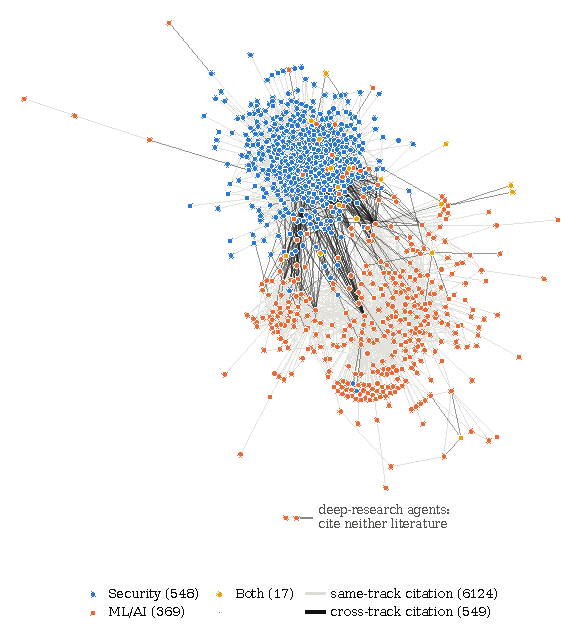
\includegraphics[width=\columnwidth]{figures/fig5_citation_network}
\caption{The corpus as a citation graph. Cross-track edges highlighted.
Papers with no resolved edge inside the corpus are omitted.}
\label{fig:network}
\end{figure}

\subsection{What has been tested against what}
\label{sec:coverage}

A (defense, attack) pair means some paper evaluated that defense against that
attack. We recovered pairs by four routes: reading defense papers, a
citation-and-full-text recovery pass, resolving benchmark names to their
constituent attacks where the paper named them, and a reverse scan of attack
papers. The last route matters because it is the only one that can observe a
defense \emph{losing} to an attack published after it. The final matrix holds
\textbf{\NPairsComposite{} confirmed pairs}.

\textbf{The matrix is sparse in a specific way.} \NDefMatchedFull{} of
\NDefenses{} defenses (\PctDefMatched{}\%) appear in at least one pair, and
\NDefOneFull{} of those (\PctDefOneFull{}\%) appear in exactly one. The
most cross-tested defense appears in \NDefCeiling{} pairs, and \NDefFourPlus{}
appear in four or more. But of the pairs belonging to those \NDefFourPlus{},
46\% were contributed by attack papers rather than by the defenses' own
evaluations; for the broadest case, seven of its eight pairs come from attack
papers. Breadth here is not evidence a method was evaluated widely by its
authors. It is evidence that attackers chose it as a target.

\textbf{How much of this gap is the field and how much is our instrument.} It
is tempting to read the complement of the matrix as ``never tested'', and that
reading is wrong. A defense evaluated on AgentDojo without naming which
injection it faced was evaluated adversarially; it is simply not a named pair,
because expanding a benchmark into its constituent attacks would manufacture
coverage. So we audited all \NDefenses{} defenses directly against their own
PDFs, asking the coarser question: was this method run against an adversary at
all? \textbf{293 (55.6\%) were}, confirmed by two independent routes that
overlap on 132 and therefore each found cases the other missed. \textbf{14
(2.7\%) report no baseline comparison of any kind}, each confirmed by hand
against the paper's own words. The remainder we report as undetermined.

We report no number drawn from a negative class, and the reason generalizes.
We built three automated passes over these papers and hand-checking each found
the same asymmetry: the positive class was reliable and the negative class was
about half wrong. A pattern can confirm that something is present in a paper;
it cannot establish that something is absent, because absence of the phrasing
it knows is not absence of the thing. \textbf{A claim that something was never
tested should state whether it means ``not done'' or ``not resolved''.}

\subsection{Who ran the experiment decides the result}
\label{sec:whoran}

For every pair we also record which side of the field reported it and what
outcome was reported.

\begin{figure}[t]
\centering
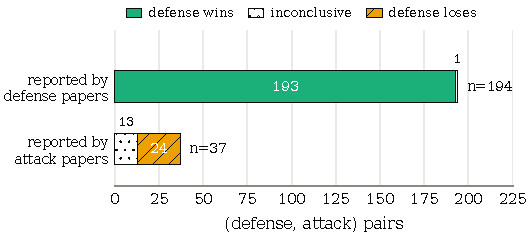
\includegraphics[width=\columnwidth]{figures/fig3_who_reports}
\caption{The same defenses and the same attacks, reported by the two sides of
the field. A defense paper reports its defense winning in \NOutcomeDefWins{}
of \NOutcomeDefPaper{} pairs. An attack paper reports the defense winning in
none of \NOutcomeAtkPaper{}.}
\label{fig:whoreports}
\end{figure}

Defense papers report their defense winning essentially always. Attack papers
report it losing essentially always. Neither number measures how often defenses
work; the pair of numbers measures publication incentive. This is why the rest
of this paper re-runs the defenses rather than citing either side's claim.

\subsection{The cell nobody has filled}
\label{sec:emptycell}

The axes so far describe what each community studies. The question this paper
turns on is narrower: \emph{has either community ever tested its methods
against the other's problems?}

We dated all \NTimelinePairs{} pairs and recorded which community each side
came from. Restricting to the \NPureTrackPairs{} pairs where both sides sit in
one of the two tracks gives Table~\ref{tab:transfer}.

\begin{table}[t]
\centering
\caption{Which community's defense met which community's attack, across
\NPureTrackPairs{} literature pairs.}
\label{tab:transfer}
\small
\begin{tabular}{@{}lrr@{}}
\toprule
defense from $\downarrow$ \quad attack from $\rightarrow$ & Security & ML/AI \\
\midrule
Security & \NSecDefSecAttack{} & \textbf{\NSecDefVsMLAttack{}} \\
ML/AI    & \NMLDefVsSecAttack{} & \NMLDefMLAttack{} \\
\bottomrule
\end{tabular}
\end{table}

\textbf{No security defense has ever been evaluated against a machine learning
failure mechanism. The cell is empty.} In the other direction there are
\NMLDefVsSecAttack{} pairs out of \NPureTrackPairs{}. Together,
\NCrossCommunityPairs{} pairs (\PctCrossCommunity{}\%) cross the boundary and
the remaining \PctSameTrack{}\% stay inside one community.

This is consistent with the citation rates and sharper than them. The
communities do not read each other, so they do not test each other, so the
question of whether either one's methods survive the other's threat model has
no answer in the published record.

\textbf{Nor is it answered by ordering.} \NDefensePredates{} of
\NTimelinePairs{} pairs (\PctDefensePredates{}\%) have a defense that predates
the attack it was tested on, so defenses do meet later attacks. But only
\NPredatesAndCross{} pair is both earlier \emph{and} cross-community.
Figure~\ref{fig:lag} shows the full distribution.

\subsection{The same ground, found twice}
\label{sec:parallel}

If two communities work one problem without reading each other, the second to
arrive restates what the first already knows. The dates say this is what
happens, and they say which direction it runs in.

\NSharedChannels{} of our nine channels have named mechanisms from both
tracks. Comparing
the first paper from each side in each of those channels:
\textbf{the security literature arrives first in \NChannelsSecFirst{} of
\NSharedChannels{}, both arrive in the same year in \NChannelsSameYear{}, and
the machine learning literature arrives first in \NChannelsMLFirst{}.} The
median lag where security leads is \MedianChannelLag{} year and the longest is
\MaxChannelLag{}. The \meth{supply-chain} channel, excluded here for having no
machine learning entry at all, is the limit case of the same pattern.

Set that beside the citation rates. A machine learning paper naming a failure
in a channel is, more often than not, naming something a security paper named
one to three years earlier, in a literature it has a
\PctMLCitesSec{}\% chance of citing. We are not claiming the later work is
derivative: these are different research questions asked of the same surface,
and arriving second at a problem is not a fault. We are claiming the obvious
consequence, which is that neither side can tell whether the other has already
answered its question, and Table~\ref{tab:transfer} shows that nobody has
checked.

Two limits on this reading. The dates are publication dates in our corpus, so
a channel that security reached first in work we did not include would move
the count. And the direction may partly reflect that security publishes
attacks, which are discrete and nameable, while the machine learning side
publishes degradations, which are noticed before they are named.

\begin{figure}[t]
\centering
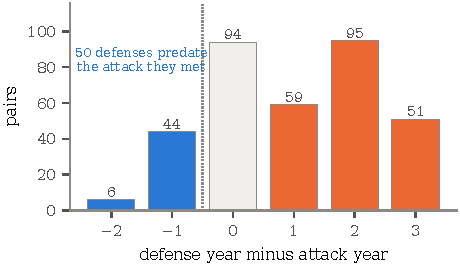
\includegraphics[width=\columnwidth]{figures/fig7_lag}
\caption{Publication lag between a defense and the attack it was tested on.}
\label{fig:lag}
\end{figure}

A reader might reasonably ask whether this is our boundary rather than the
field's. We assign the track label per paper. Papers that sit on the boundary are
coded ``Both'' and excluded from Table~\ref{tab:transfer}, because a paper
cannot cross a line it sits on. Including them gives
\NCrossAllPairs{} of \NTimelinePairs{} rather than
\NCrossCommunityPairs{} of \NPureTrackPairs{}, and the empty cell stays empty
either way.

\textbf{The rest of this paper fills that cell.}
